\myparagraph{Le nano-ordinateur}
\noindent L'objet d'étude de cet essai est le nano-ordinateur "Jetson Nano" du fabricant "NVIDIA" (figure \ref{fig:jetson_nano_lego}). Ce modèle a été choisi car il a été conçu par la compagnie NVIDIA spécifiquement pour répondre au besoin d'inférence en temps réel sur le terrain, afin d'éviter le transfert de données et le traitement à distance et différé. 
\begin{figure}[H]
    \centering
    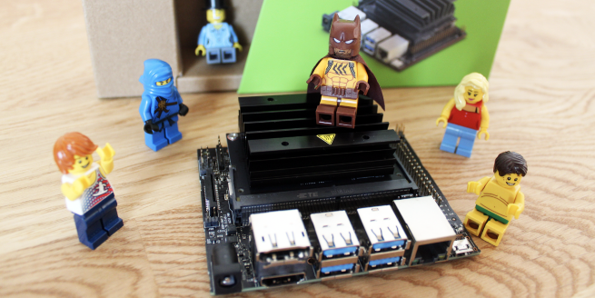
\includegraphics[width=0.75\textwidth]{jetson_nano_lego}
    \caption[Carte mère Jetson Nano de NVIDIA]{Carte mère Jetson Nano de NVIDIA, représenté avec des Lego pour démontrer sa petite taille}
    \label{fig:jetson_nano_lego}
\end{figure}
\noindent L'architecture du nano-ordinateur est ARM 64 bits (aarch64), ce qui le limite pour certaines portabilités de librairies, surtout dans le domaine assez restreint de la recherche, ou l'architecture la plus populaire et portable est x86-64. Il est composé d'un quad-core ARM Cortex-A57 @ 1.43 GHz, qui est conçu pour ce genre de nano-ordinateur, comme le Raspberry Pi. Les performances \acrshort{gpu} du Maxwell sont de 128-cores @ 921 MHz, 0.5 \acrshort{tflops} (16 FP = 16 bits FP = 2 bytes Floating Points). Par comparaison la PlayStation 4 Pro (2016) supporte +4 \acrshort{tflops}. La mémoire est limitée à 4Gb LPDDR4 @ 1.6 GHz. Les autres caractéristiques à considérer sont le port pour une carte microSD, un port Ethernet 10/100/1000Mbs, un port HDMI, un hub USB 4 ports 3.0, un connecteur pour une caméra, et un port PCIe. Le tout tient sur une carte mère d'une taille de 69.6 mm x 45 mm, et consomme entre 5 et 10 watt.
\myparagraph{Logiciels}
\vspace{0.5\baselineskip}
\\
\noindent De même que pour les périphériques, les solutions logiciels principales qui sont utilisés dans le cadre de l'essai sont résumés dans le tableau suivant, où il est indiqué leur nom, le type de licence, leur version, leurs rôles et responsabilités, comme pour le système d'exploitation, l'environnement de développement pour l'apprentissage profond, l'inférence, les logiciels de traitements vidéos et d'images. 
\vspace{0.5\baselineskip}
\\
\noindent Pour tester les performances de la microSD et du disque SDD interne M.2 NVMe, l'utilitaire "hdparm" a été utilisé. 
\vspace{0.5\baselineskip}
\\
\noindent Le \acrshort{sdk} qui est utilisé avec le nano-ordinateur est celui fourni par NVIDIA et qui se nomme "JetPack"\footnote{\url{https://developer.nvidia.com/embedded/jetpack}} \footnote{\url{https://docs.nvidia.com/jetson/jetpack/introduction/index.html}}. La version 4.4\footnote{\url{https://developer.nvidia.com/embedded/jetpack-archive}} est celle avec laquelle les tests de performance ont été exécutés. Il contient le système d'exploitation "\acrlong{l4t}" (\acrshort{l4t})\footnote{\url{https://developer.nvidia.com/embedded/linux-tegra}} (version \acrshort{l4t} 32.4.3), qui est une version de la distribution Linux Ubuntu 18.04 mise à la saveur de NVIDIA. Jetpack contient aussi d'autres librairies qui sont nécessaires pour re construire la version \acrshort{onnx} du modèle, tel que Cuda, CuDNN et TensorRT.
\begin{figure}[H]
    \centering
    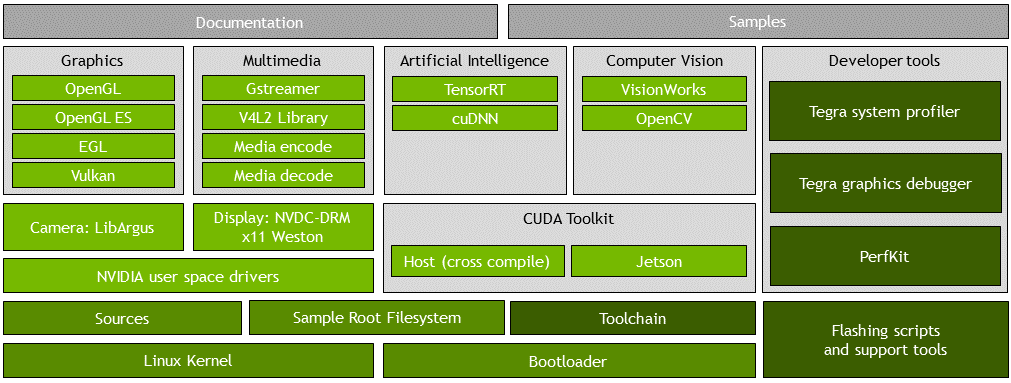
\includegraphics[width=1.0\textwidth]{jetpack_architecture}
    \caption[Diagramme de l'architecture du NVIDIA JetPack]{Diagramme de l'architecture du NVIDIA JetPack\protect\footnotemark}
    \label{fig:jetpack_architecture}
\end{figure}
\footnotetext{\url{https://docs.nvidia.com/jetson/l4t/index.html#page/Tegra\%2520Linux\%2520Driver\%2520Package\%2520Development\%2520Guide\%2Foverview.html\%23}}
\noindent Python et C++ sont les langages utilisés par la plateforme applicative de DeepLearning de NVIDIA. Python est utilisé comme langage accessible et appelle les extensions écrites en C++ et qui optimisent les accès aux ressources systèmes tel que les \acrshort{cpu}s et \acrshort{gpu}s, les traitements des images et vidéos, les boucles et les traitements mémoires intensifs.
\vspace{0.5\baselineskip}
\\
\noindent La librairie d’apprentissage profond qui est utilisée est PyTorch, bonifié avec une version adaptée par NVIDIA de torchvision, qui fournit des architectures et des utilitaires pour la vision par ordinateur (computer vision). Des versions bien spécifiques sont nécessaires et il est important de s'y conformer au risque de tomber dans une investigation bien couteuse en temps et énergie\footnote{\url{https://forums.developer.nvidia.com/t/trying-to-regenerate-onnx-for-jetson-nano/125494?u=vincelf}}.
\vspace{0.5\baselineskip}
\\
\noindent Le nano-ordinateur inclut un \acrshort{gpu} qui est mis à contribution lors de l'inférence. Le compilateur de NVIDIA pour \acrshort{gpu} 'cuda' est nécessaire pour regénérer la version \acrshort{onnx}. La version doit concorder avec la bonne version de PyTorch. La version adaptée (fork) de torchvision doit être recompilée avec la bonne version de pytorch et cuda. 
\vspace{0.5\baselineskip}
\\
\noindent Enfin pour regénérer la version \acrshort{onnx} lors de la phase de réentrainement, les librairies TensorRT et \acrshort{onnx} ont été utilisées, en compagnie de l'utilitaire `trtexec` qui permet de valider et tester le fichier \acrshort{onnx} généré.
\vspace{0.5\baselineskip}
{
    \vspace{0.1em} % Adjust the height of the space between caption and tabular
    \begin{longtable}[t]{{@{}|p{5em}|p{3em}|p{4em}|p{23em}|@{}}} % p{15em}p{35em} with landscape
        \caption{Solutions logicielles de l'essai}\label{table:table_sol_logiciel}\\
        \hline
        \textbf{Language} & \textbf{Version} & \textbf{Licence} & \textbf{Rôles et responsabilités} \\
        \endfirsthead
        \hline
        \textbf{Language} & \textbf{Version} & \textbf{Licence} & \textbf{Rôles et responsabilités} \\
        \hline
        \endhead
        \endfoot
        \endlastfoot
        \hline
        JetpPack & 4.4 & NVIDIA & Kit de développement de logiciels incluant le système d'exploitation \acrshort{l4t}, et les librairies et utilitaires nécessaires pour l'inférence avec le nano-ordinateur.\\
        \hline
        \acrshort{l4t} & 32.4.3 & NVIDIA & Le système d'exploitation "\acrlong{l4t}" conçut par NVIDIA pour leurs solutions d'inférence légères, comme pour le nano-ordinateur.\\
        \hline
        Python & 2.7 & GPL & Language plus accessible que le C++.\\
        \hline
        C++ (gcc) & 7.3.1\footnote{\url{https://developer.nvidia.com/embedded/linux-tegra}} & GPL & Certaines extensions du cadre applicatif de NVIDIA pour l'inférence sont écrites en C++, pour des raisons d'optimisation.\\
        \hline
        pytorch & 1.1.0 & BSD 3-Clause & Cadre de développement d'application pour l'apprentissage machine et profond.\\
        \hline
        torchvision & 0.0.3 & BSD 3-Clause & Branche de torchvision adaptée par NVIDIA\footnote{\url{https://github.com/dusty-nv/vision.git} et ensuite branche v0.3.0}; Doit être recompilée avec la version de pytorch 1.1.0 et cuda 10.0.\\
        \hline
        cuda & 10.0 & NVIDIA & Compilateur de code C++ pour \acrshort{gpu}.\\
        \hline
        TensorRT & 6.0.1.5 & NVIDIA & \acrshort{sdk} pour générer des modèles au format \acrshort{onnx}, optimisés et interopérables, pour l'inférence.\\
        \hline
        \acrshort{onnx} & 1.7.0 & MIT & Librairie qui permet de générer un format interopérable pour l'inférence de modèles d'architecture construits avec différente plateforme applicative d'apprentissage machine (Caffe, PyTorch, TensorFlow, etc.).\\
        \hline
        trtexec & - & NVIDIA & Utilitaire qui a permis de tester la version \acrshort{onnx} qui a été regénéré.\\
        \hline
        gstreamer & 1.14.5 & LGPL & Utilitaire qui a permis d'alimenter l'architecture de la segmentation avec la vidéo.\\
        \hline
        v4l2loopback & 0.12.5 & GPL & Utilitaire qui a permis de créer un matériel vidéo virtuelle permettant de remplacer la caméra, permettant ainsi au modèle d'être alimenté par une vidéo et non la caméra. Une fois installé, le matériel vidéo virtuel est accessible via "/dev/video1", "/dev/video0" étant réservé pour la caméra. \\
        \hline
        hdparm & 9.54 & GPL & Utilitaire permettant de tester la capacité de lecture d'une unité de stockage, tel que'un \acrshort{ssd} NVMe et différentes cartes microSD.\\
        \hline
        tegrastats & - & NVIDIA & La commande offre différents indicateurs système tel que l'utilisation des processeurs, la température, la consommation, et qui sont utiles pour observer le comportement du système lors des tests de performance de la segmentation.\\
        \hline
        free & 3.3.12 & GPL & La commande offre le statut de la mémoire totale, utilisée, libre, swap, cachée, etc. Elle est utile pour observer le comportement de la mémoire du nano-ordinateur lors des tests de performance de la segmentation.\\
        \hline
        iotop & 0.6 & GPL & La commande offre le statut des opérations "I/O" de lecture \& écriture sur le disque, totale ou pour le processus de segmentation. Elle est utile pour observer le comportement des opérations sur le disque du nano-ordinateur lors des tests de performance de la segmentation.\\
        \hline
        segnet-console & - & NVIDIA & La commande permet de segmenter une image. L'architecture est donnée en argument. Lors de l'essai, celle qui a été évaluée est "fcn-resnet18-deepscene-576x320". Les options qui doivent être utilisées pour que l'image générée soit évaluée doivent être "-{}-visualize=mask -{}-filter-mode=point -{}-alpha=0". L'image originale est fournie en avant-dernière place de la commande, et l'image générée en dernière place. Il est possible aussi de démarrer l'inférence avec sa propre architecture grâce aux options "-{}-model", "-{}-prototxt", "-{}-labels", "-{}-colors", "-{}-input\_blob" et "-{}-output\_blob".\\
        \hline
        segnet-camera & - & NVIDIA & La commande permet de démarrer la segmentation avec la caméra, ou optionnellement avec un matériel vidéo virtuel (fournie par "v4l2loopback") grâce à l'option "-{}-camera=/dev/video1", comme cela a été le cas durant le projet pour évaluer la segmentation avec des vidéos au lieu de la caméra. L'architecture est donnée en argument. Lors de l'essai, celle qui a été évaluée est "fcn-resnet18-deepscene-576x320". La résolution peut être précisée grâce aux options "width" et "height", mais durant l'évaluation les valeurs par défaut ont été conservées (width=1280px et height=720px). Il est possible aussi de démarrer l'inférence avec sa propre architecture grâce aux options "-{}-model", "-{}-prototxt", "-{}-labels", "-{}-colors", "-{}-input\_blob" et -{}-output\_blob". Il n'est pas possible de conserver la vidéo segmentée, et il n'est pas possible de sauvegarder les images qui sont rafraichies à l'écran dans la fenêtre XWindow car le code nécessaire à cette sauvegarde est trop intrusif et impacte négativement les performances de la segmentation et du nano-ordinateur. L'évaluation des performances n'est donc que visuelle, et cette limitation pourrait remettre en question le désir de détecter les délimitations de la piste cyclable en temps réel, puisqu'il n'y a pas de moyen de récupérer le résultat généré.\\
        \hline
    \end{longtable}
}
% \clearpage
% \newpage